\documentclass[11pt]{article} % use larger type; default would be 10pt

\usepackage[utf8]{inputenc} % set input encoding (not needed with XeLaTeX)
\usepackage{siunitx}
\usepackage{amsmath}
\usepackage{graphicx}

%%% Examples of Article customizations
% These packages are optional, depending whether you want the features they provide.
% See the LaTeX Companion or other references for full information.

%%% PAGE DIMENSIONS
\usepackage{geometry} % to change the page dimensions
\geometry{a4paper} % or letterpaper (US) or a5paper or....
% \geometry{margin=2in} % for example, change the margins to 2 inches all round
% \geometry{landscape} % set up the page for landscape
%   read geometry.pdf for detailed page layout information

\usepackage{graphicx} % support the \includegraphics command and options

% \usepackage[parfill]{parskip} % Activate to begin paragraphs with an empty line rather than an indent

%%% PACKAGES
\usepackage{booktabs} % for much better looking tables
\usepackage{array} % for better arrays (eg matrices) in maths
\usepackage{paralist} % very flexible & customisable lists (eg. enumerate/itemize, etc.)
\usepackage{verbatim} % adds environment for commenting out blocks of text & for better verbatim
\usepackage{subfig} % make it possible to include more than one captioned figure/table in a single float
% These packages are all incorporated in the memoir class to one degree or another...

%%% HEADERS & FOOTERS
\usepackage{fancyhdr} % This should be set AFTER setting up the page geometry
\pagestyle{fancy} % options: empty , plain , fancy
\renewcommand{\headrulewidth}{0pt} % customise the layout...
\lhead{}\chead{}\rhead{}
\lfoot{}\cfoot{\thepage}\rfoot{}

%%% SECTION TITLE APPEARANCE
\usepackage{sectsty}
\allsectionsfont{\sffamily\mdseries\upshape} % (See the fntguide.pdf for font help)
% (This matches ConTeXt defaults)

%%% ToC (table of contents) APPEARANCE
\usepackage[nottoc,notlof,notlot]{tocbibind} % Put the bibliography in the ToC
\usepackage[titles,subfigure]{tocloft} % Alter the style of the Table of Contents
\renewcommand{\cftsecfont}{\rmfamily\mdseries\upshape}
\renewcommand{\cftsecpagefont}{\rmfamily\mdseries\upshape} % No bold!

%%% END Article customizations

%%% The "real" document content comes below...

\title{LightForm Surfalex Experimental Report}
\author{Sumeet Mishra, Peter Crowther}
\date{} % Activate to display a given date or no date (if empty),
         % otherwise the current date is printed 

\begin{document}
\maketitle

\section{Introduction}
In the present work, an AA 6016 alloy which is denoted by the name ‘Surfalex’ was used as a model material to develop a robust framework for numerical simulations of formability. In this regard, an extensive experimental data set consisting of material properties such as yield strength, work hardening behaviour, Lankford parameter and grain morphology and texture was developed by performing uniaxial tensile tests, forming limit tests and electron back scatter diffraction (EBSD). It should be noted that the uniaxial tensile tests and forming limit tests were performed in combination with digital image correlation (DIC) to obtain the full strain paths (transverse and axial strain) during plastic deformation. The extensive data set enabled the determination of crystal plasticity parameters which were then subsequently used to simulate yield surface and the forming limit curve. 

\section{Material and experimenal methodology}
The Surfalex material was provided by provided by M/s Constellium, France. The composition of the Surfalex material is provided in Table \ref{tab:compositon}. The thickness of the Surfalex sheet was \SI{1.5}{\milli\meter}. 

\begin{table}[]
\begin{tabular}{|l|l|l|l|l|l|l|l|l|}
\hline
Si             & Fe             & Cu             & Mn             & Mg      & Cr             & Zn             & Ti              & Al   \\ \hline
\textless{}1.5 & \textless{}0.5 & \textless{}0.2 & \textless{}0.2 & 0.2-0.6 & \textless{}0.1 & \textless{}0.2 & \textless{}0.15 & Rest \\ \hline
\end{tabular}
\caption{Composition (in wt\%) of AA 6016 Surfalex material}
\label{tab:compositon}
\end{table}

\subsection{Tensile testing with DIC}
Tensile testing with two-dimensional digital image correlation was performed at room temperature using an Instron universal testing machine (UTM) with \SI{5}{\kilo\newton} load cell and a Strain Master DIC system by LaVision. Images were captured for every one second (\SI{1}{\hertz}) which were then subsequently used for digital image correlation. The tensile tests were performed at a constant strain rate of \SI{5e-4}{\per\second}. The dimensions of tensile specimen are shown in Fig. \ref{fig:dic_specimens}a. It should be noted that the tensile specimens were prepared along different orientations with respect to the rolling direction to estimate the anisotropy in mechanical properties (Fig. \ref{fig:dic_specimens}b). The tensile specimens were polished followed by thorough cleaning to obtain a contamination free surface. The clean surface was then spray painted with a white primer coat followed by a top layer of black speckles to obtain the necessary contrast for image correlation. Fig. \ref{fig:dic_specimens}c shows a typical image of the speckle pattern that was used in the current work. It was ensured that the speckled surface was properly illuminated during the test to obtain a high contrast which important for subsequent processing of images.

\begin{figure}[h]
	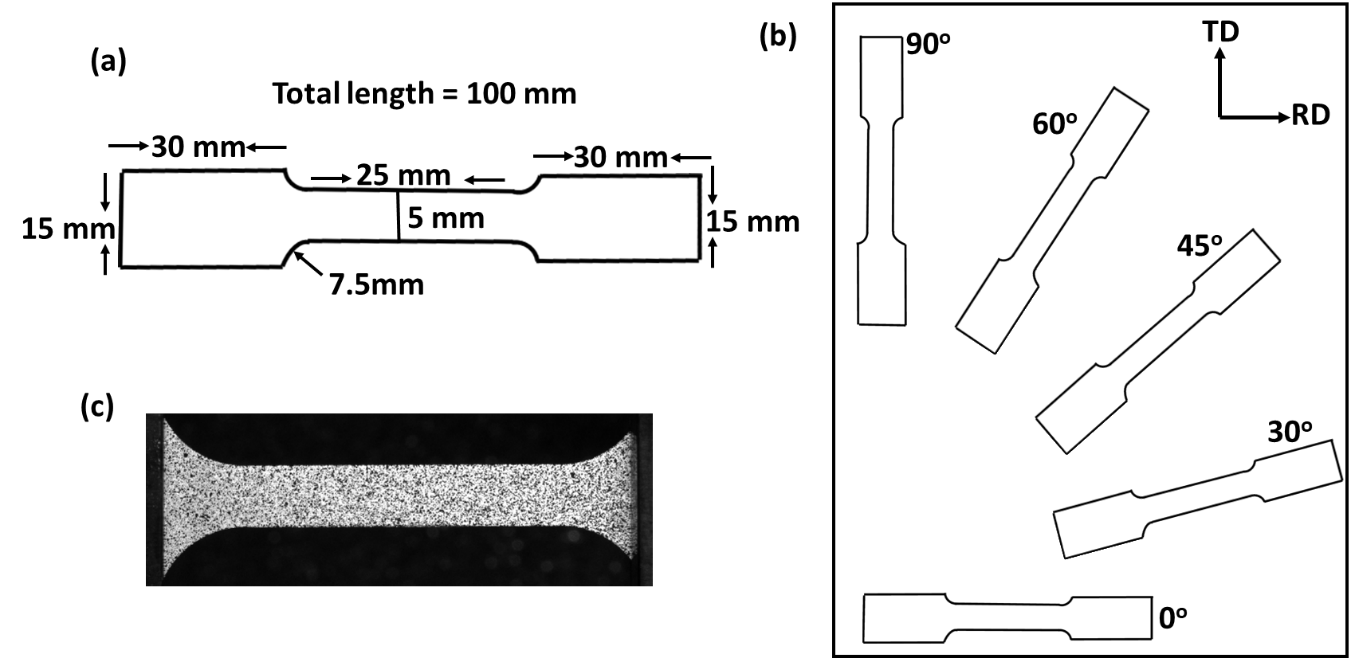
\includegraphics{figures/dic_specimens}
	\centering
	\caption{(a) Dimensions of the tensile specimen (b) Different orientation of tensile specimens with respect to rolling direction (RD) (c) Speckle pattern on the gauge length of a representative tensile
 sample.
	\label{fig:dic_specimens}}
\end{figure}

Following the tensile tests, image correlation was performed using LaVision DaVis software version 10. The correlation was performed using a subset size of 31 pixels, step size of 10 pixels and correlation method of ‘relative to the first’. A step size which is 1/3rd of the subset size was chosen to have a decent spatial resolution. Following the correlation, displacement data from DaVis software was exported as ‘.csv’ files for further analysis and visualization using an in house developed Python script. The displacement data was used to calculate the individual components of the displacement gradient tensor ($e$) in the x1-x2 reference frame.
\begin{equation}
	e = \begin{bmatrix}
			\frac{\partial u}{\partial x} & \frac{\partial u}{\partial y} \\ 
			\frac{\partial v}{\partial x} & \frac{\partial v}{\partial y}
		\end{bmatrix}
\end{equation}
Here the strain component $\frac{\partial v}{\partial y}$ corresponds to strain along the axial direction while $\frac{\partial u}{\partial x}$ is the transverse strain. The magnitude of components $\frac{\partial u}{\partial y}$ and $\frac{\partial v}{\partial x}$ was observed to be several orders of magnitude smaller compared to $\frac{\partial v}{\partial y}$ and $\frac{\partial u}{\partial x}$. Apart from the strain, the load cell output from Instron UTM which in in voltage was also recorded by the DaVis softeware. The voltage was subsequently converted to load using the conversion formula of \SI{1}{\volt} = \SI{0.5}{\kilo\newton}. This facilitated the determination of precise stress versus strain curves which is free of errors such as machine compliance. 

\subsection{Nakazima forming limit tests with DIC}
In the present work, Nakazima tests were carried out to construct the forming limit curve of Surfalex material. A diagram of the hemispherical punch is shown in Fig. \ref{fig:punch}. The diameter punch was \SI{177}{\milli\meter}, the fillet raidus was \SI{30}{\milli\meter}, the shaft length was \SI{50}{\milli\meter} and the shaft width . As can be observed, a range of sample widths varying from \SI{10}{\milli\meter} to \SI{177}{\milli\meter} was employed for Nakazima tests. This was to mimic different strain paths such as uniaxial, plain strain and biaxial conditions (Fig \ref{fig:strain_path}). In a process similar to that of tensile testing, the Nakazima samples were also cleaned thoroughly and then spray painted with a white primer coat followed by a top layer of black speckles to facilitate strain measurement via image correlation technique. Graphite was used as lubricant for all the tests and was applied to that side of the sample which comes in contact with the punch. Sufficient time was given for the spray paint to dry out following which the samples were turned over and graphite lubricant was applied with a brush. This ensured that the speckle pattern remained intact and was not damaged by the lubricant. The punch speed was maintained at \SI{1}{\milli\meter\per\minute} for all the tests. The clamp force of \SI{200}{\kilo\newton} was used so as to ensure that the samples did not slip during the tests. Images were continuously acquired during the tests using the GOM-ARAMIS set up to obtain the displacement data. The images were captured for every \SI{0.5}{\second} for the first \SI{25}{\second}. After that, the acquisition frequency was increased and images were captured for every \SI{0.05}{\second} until the end of the test. 

\begin{figure}[h]
	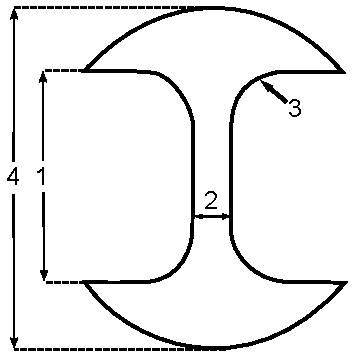
\includegraphics{figures/nakazima_punch}
	\centering
	\caption{Diagram of Nakazima punch. Distance 1 is the shaft length, 2 is the blank width, 3 is the filler radius and 4 is the sample diameter.}
	\label{fig:punch}
\end{figure}

Following the tests, image correlation was performed using GOM Correlate Professional 2019. Firstly, a surface component was created using a facet size of 19 pixels and point distance of 16 pixels which ensured maximum surface coverage. The first image which was acquired several frames prior to the contact of punch with the sample was used as the reference image, against which all the other strain calculations were compared. It was ensured that strain representation is always kept as true strain instead of other options such as technical strain, stretch ratio and green strain. Following the determination of strain, major and minor strains were calculated using the GOM Correlate software. The calculation of major and minor strains involves principal axis transformation of the strain tensor to provide the eigen values and eigen vectors. The larger eigen value corresponds to major strain while the smaller eigen value corresponds to minor strain. Following the calculation of major and minor strains, a fully automated FLC script embedded in the GOM Correlate environment was used to set up three sections perpendicular to the crack direction and export the major and minor strains in the right format for further analysis and computation. It should be noted that the three sections are denoted as ‘section zero’, ‘section one’ and ‘section two’, respectively. The spacing between the sections was kept at \SI{2}{\milli\meter} in accordance with the ISO12004 standard. In the following paragraph a brief explanation of the working of FLC script will be provided.  


The first step in the FLC script is to identify the stage at which the crack forms. This step is followed by locating the position of crack by further probing the particular ‘stage of interest’. In order to perform these steps, the FLC script utilizes out of the plane velocity or velocity in z direction (Vz). Since the punch speed was maintained at \SI{1}{\milli\meter\per\second}, it can be envisioned that velocity in ‘z’ direction would also be close to \SI{1}{\milli\meter\per\second} as the test specimen wraps around the hemispherical punch. However, when the crack will appear there will be a sudden increase in velocity. This is shown in Fig. 4 for several stages of a representative test. As can be observed, for all the stages prior to crack formation, velocity in z direction remains at \SI{1}{\milli\meter\per\second}. However, when the crack appears there is a sudden jump from \SI{1}{\milli\meter\per\second} to \SI{20}{\milli\meter\per\second}. Moreover, the particular location on sample where the crack forms can also be identified from Fig. 4h. Once the crack location is found, the script sets up three sections which are perpendicular to the crack direction (Fig. 5) and exports the major and minor strain data (.csv files) across these section for all stages starting from the beginning to the end of the test. The major and minor strain data can found using the following link (Provide the link here).  

\begin{figure}[h]
	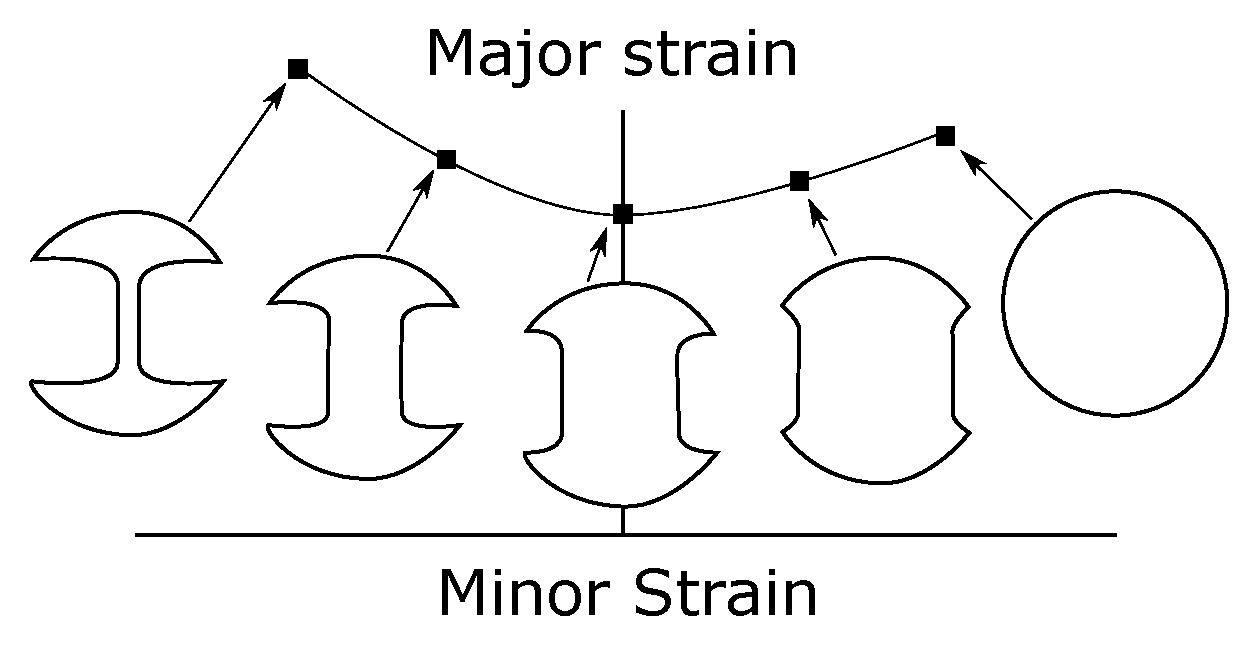
\includegraphics[width=\textwidth]{figures/strain_path}
	\centering
	\caption{Schematic of forming limit curve highlighting the different strain paths that can be achieved with different sample widths.}
	\label{fig:strain_path}
\end{figure}


\subsection{Electron back scatter detection (EBSD)}
In order to determine the crystallographic texture and grain morphology of Surfalex material, EBSD was carried out using a FEI Sirion field emission gun scanning electron microscope equipped with Nordlys detector from Oxford instruments. An acceleration voltage of \SI{20}{\kilo\volt}, working distance of \SI{16}{\milli\meter} and step size of \SI{2}{\micro\meter} was used to capture large area EBSD scans. The large areas ensured that sufficient number of grains were captured for a reliable estimate of texture. It should be noted that EBSD scans were performed on three different planes viz. RD-TD, RD-ND and TD-ND planes to get an accurate information about through thickness variation in grain morphology and texture (Fig. 6). Moreover, EBSD scans on different planes facilitated the preparation of representative volume element which was subsequently used for performing crystal plasticity simulations. The EBSD data analysis to obtain the inverse pole figure maps, pole figures and orientation distribution function (ODF) was performed using MTEX software. For the EBSD scans performed on the RD-ND and TD-planes, the data was appropriately rotated (by \ang{90} about the ‘x’ axis) to represent the maps and pole figures in correct reference frame. 


The sample preparation for EBSD involved the standard grinding steps from 600 grit to 4000 grit followed by \SI{3}{\micro\meter} and \SI{1}{\micro\meter} diamond polishing. The final stage of polishing involved the use of colloidal silica with a particle size of \SI{0.02}{\micro\meter} µm. In order to ensure good surface quality, the samples were further subjected to electropolishing using a solution of 70\% methanol and 30\% nitric acid. It was ensured that the electrolyte was kept at \SI{-15}{\celsius} during the entire process. The polishing voltage and time were \SI{10}{\volt} and \SI{10}{\second}, respectively. 

\begin{figure}[h]
	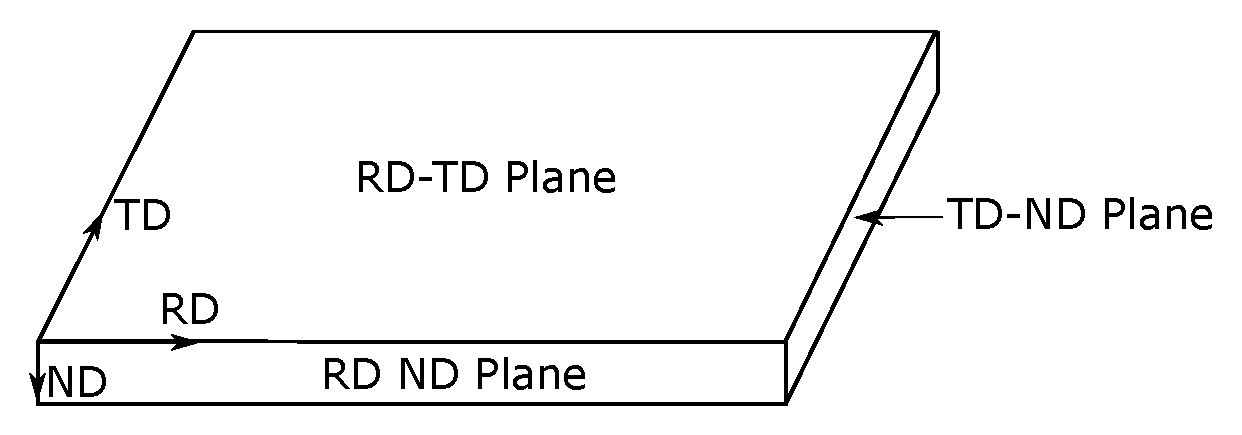
\includegraphics[width=\textwidth]{figures/sample_orientations}
	\centering
	\caption{Schematic showing the different planes on which EBSD scans was performed. The EBSD scans taken on RD-ND and TD-ND plane were rotated by 90 degrees to accurately represent the texture and microstructure.}
	\label{fig:orientations}
\end{figure}


\section{Overview of necking criteria}
In the past, several necking criterias have been used to predict the onset of localised neck formation in Nakazima test samples. In the present work, we have employed time dependent criterias which are based on the evolution of major strain and major strain rate at some specific points on the specimen. A brief overview of the different necking criterias is provided below.

\subsection{Second derivative criteria}
This criterion is based on abrupt change in major strain rate at a point in the neck region \cite{Song2019}. As the localised neck forms and starts to propagate, the major strain will localise within the neck. Consequently, the major strain rate will increase at a much faster rate. Therefore, the onset of necking is detected when the 2nd derivative of the major strain in the neck starts to deviate from a constant value.  However, in actual situations there is never an abrupt deviation from the constant value. Instead, there is a gradual transition. Therefore, a threshold criterion has to be used to detect the onset of necking. In the present work, a threshold of 10\% of the maximum value of 2nd derivative of the major strain was used to detect the formation of neck. The different steps of this 2nd derivative criteria are shown in Fig. 7 for a representative sample. 

\subsection{Incremental strain in the neck and away from neck region}
This criterion is based on the skeleton structure of the well-known Marciniak-Kuczynski (MK) model which is used widely for predicting forming limit curves of engineering metals and alloys \cite{Banabic2010}. The MK model assumes a defect in terms of a region of reduced thickness (Fig\ref{fig:mk_flaw}) being present in the sample. A key assumption of the MK model is that when necking occurs, the major strain increment in the neck region and away from the neck region will be greater than 10\cite{Narasimhan1991}. In this regard, the evolution of major strain rate with time was analysed for points in the neck and away from the neck region and their ratio was tracked. The time at which the ratio exceeded 10 was chosen as the onset of necking. The different steps of this necking criteria are shown in Fig. 9. An additional benefit of using this criterion is that it is consistent with our finite element simulations where MK method along with constitutive relationships and yield criterias are implemented to predict the forming limit curve of the Surfalex material.   

\begin{figure}[h]
	
\includegraphics[width=\textwidth]{figures/mk_flaw}
	\centering
	\caption{Schematic of a presence of small flaw of reduced thickness $t_b$ compared to overall sheet thickness $t_a$ as assumed in the Marciniak-Kuczynski model.}
	\label{fig:mk_flaw}
\end{figure}

\section{Experimental Results}
\subsection{Initial microstructure and texture}
The inverse pole figure maps (Z direction) illustrating the microstructure of Surfalex material on RD-TD, RD-ND and TD-ND planes are shown in Fig. 10. The microstructure can be characterized by the presence of more or less equiaxed grains with an average grain size of 30 µm. The average aspect ratio of grains was found to be ~1.5 which confirms the equiaxed nature of the grains. In addition, it can also be observed that there is no orientation gradient present within the individual grains. The Kernel average misorientation maps were also verified from which it was confirmed that Surfalex material is in a soft annealed condition with negligible residual strain. 
The crystallographic texture of the Surfalex material is shown in Fig. 11 in terms of (111), (200) and (220) pole figures. It can be observed that a well-defined Cube texture {001} <001> is present in the Surfalex material, irrespective of the plane on which texture measurements were carried out. Considering that Cube texture is typically observed in Al alloys after recrystallization annealing treatment, it can be again confirmed that Surfalex material is in a recrystallized or ‘O’ temper condition. The maximum intensity in the pole figures is ~3.5 x random which signifies that the texture in Surfalex material is not very sharp.  

\subsection{Mechanical properties and Lankford parameter}
The results of uniaxial tensile tests performed along several directions from rolling direction are shown in Fig. 12 (a-b). It can be observed that direction dependency of mechanical properties such as yield and ultimate tensile strength is relatively weak. This can be attributed to weak texture of Surfalex material. Another important property viz. Lankford parameter (strain in width/strain in thickness) was determined using the digital image correlation technique (Fig. 12b). In order to determine Lankford parameter, the parameter $\rho$ which is the ratio of transverse to axial strain was determined first following which the subsequent equation was used to calculate Lankford parameter ($R$).  
\begin{equation}
	R = \frac{\rho}{1-\rho}, \;\;\; \rho = -\frac{transverse\:strain}{axial\:strain}
\end{equation}
Here, the concept of volume constancy during plastic deformation is used to derive the strain along thickness direction using the in-plane axial and transverse strains. It can be observed from Fig. 12b that Lankford parameter is higher along 0 and 90 degrees from RD compared to 45 degrees from RD. This trend is a characteristic signature of Cube texture and has been observed previously by several researchers in the past\cite{Engler2015}.  

The evolution of strain distribution across the gauge length is shown in Fig. \ref{fig:strain_maps} for some representative tensile samples along a) 0, b) 45 andd c) \ang{90} from RD. It can be observed that there is no marked dependency of strain localisation or the necking characteristics with orientation of tensile axis. This behaviour can again be attributed to the weak texture present in Surfalex material. 

\begin{figure}[h]
	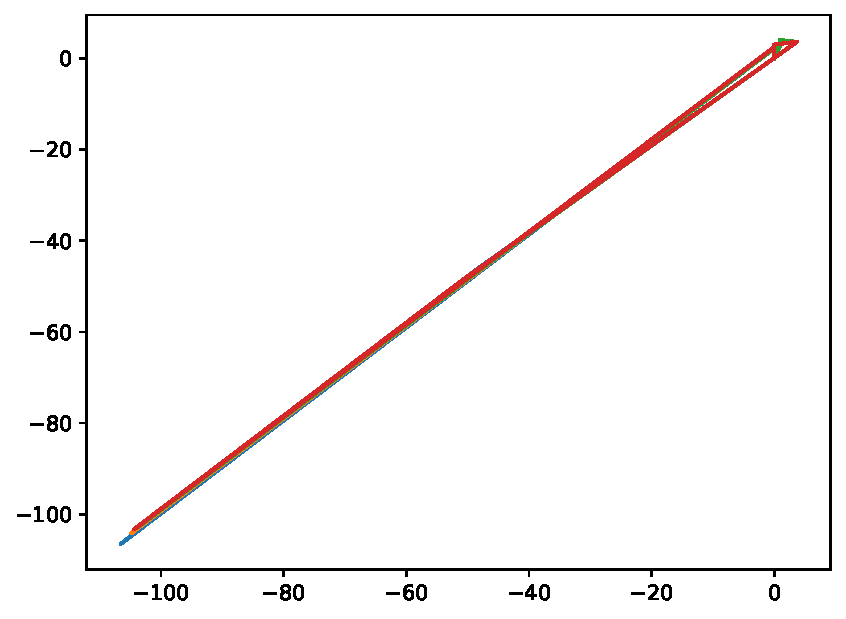
\includegraphics[width=\textwidth]{figures/strain_maps}
	\centering
	\caption{Strain maps across the gauge length of the tensile samples at different stages (from beginning to the end) (a) Parallel to RD (b) \ang{45} to RD (c) \ang{90} to RD. Numbers above each map give the timestep of the map.}
	\label{fig:strain_maps}
\end{figure}

\subsection{Forming limit curve}
Fig. 14 shows the forming limit strains for the Surfalex material obtained using the two necking criterias discussed in Section 3 viz. 2nd derivative method and major strain rate ratio method. It can be observed that major strain rate ratio method is more conservative compared to second derivative method. For all the different strain paths, 2nd derivative method predicts higher limit strains compared to major strain rate ratio method. It should be noted that in Nakazima tests, data points are typically shifted towards the biaxial stretching region due to the interaction of hemispherical punch with the sample. However, the biaxial stretching is more prevalent in the central part of the Nakazima samples compared to its ends. Nonetheless, in the present case, crack appears at the end of the gauge length for the representative Surfalex sample (Fig. 5). The appearance of crack at the end of the gauge length was observed to be occurring for all the Nakazima samples of different width. Therefore, the effects of non-proportional strain path or shifting of data points towards the biaxial regime is less prevalent in the Surfalex material. 


\bibliographystyle{unsrt}
\bibliography{experimental_report}
\end{document}
